%%% -*- TeX-master: "../main" -*-
\chapter{Results}
\label{cha:results}

% TODO: Discussion of why frame reconstruction did not work?

\begin{figure}[h]
  \begin{subfigure}{3in}
  \centering
    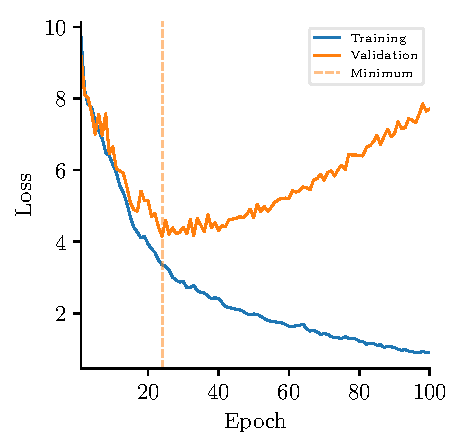
\includegraphics[width=3in]{figures/results/losses/gru-gists}
    \caption{Cross Entropy}
  \end{subfigure}
  \hfill
  \begin{subfigure}{3in}
  \centering
    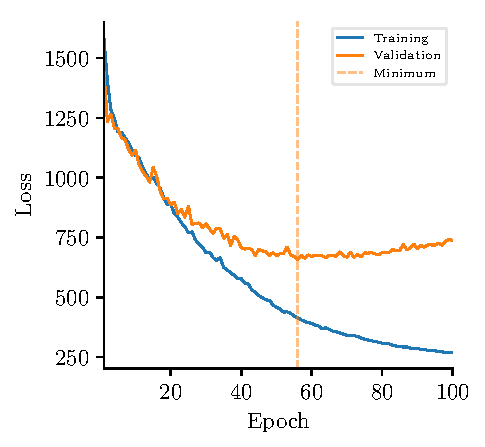
\includegraphics[width=3in]{figures/results/losses/ctc-gists}
    \caption{CTC}
  \end{subfigure}
  \caption{}
  \label{fig:loss-gists}
\end{figure}

\begin{figure}[h]
  \begin{subfigure}{3in}
  \centering
    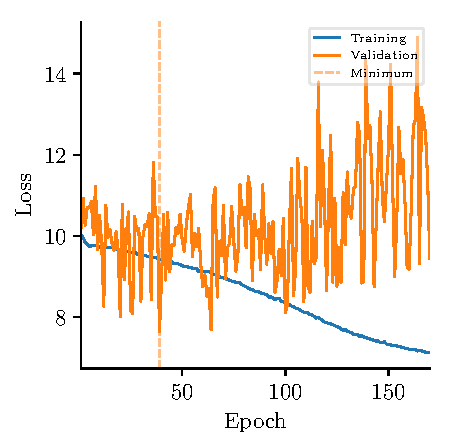
\includegraphics[width=3in]{figures/results/losses/gru-inceptionv3}
    \caption{Cross Entropy}
  \end{subfigure}
  \hfill
  \begin{subfigure}{3in}
  \centering
    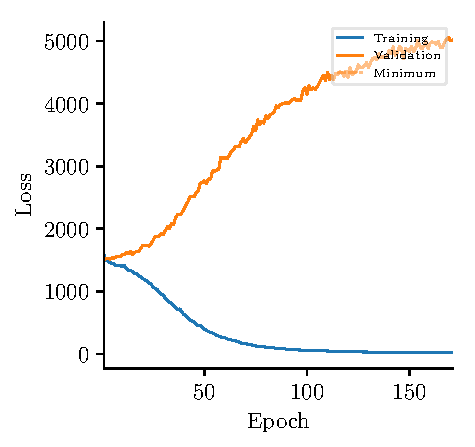
\includegraphics[width=3in]{figures/results/losses/ctc-inceptionv3}
    \caption{CTC}
  \end{subfigure}
  \caption{}
  \label{fig:loss-inceptionv3}
\end{figure}

\begin{figure}[h]
  \begin{subfigure}{3in}
  \centering
    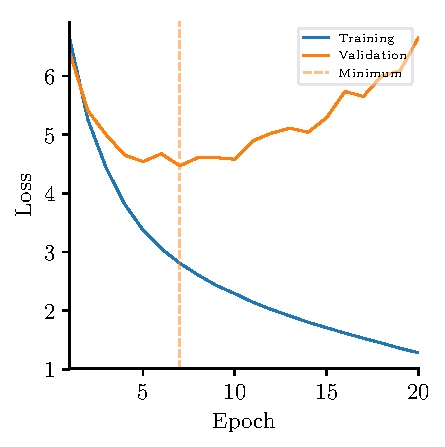
\includegraphics[width=3in]{figures/results/losses/gru-events}
    \caption{Cross Entropy}
  \end{subfigure}
  \hfill
  \begin{subfigure}{3in}
  \centering
    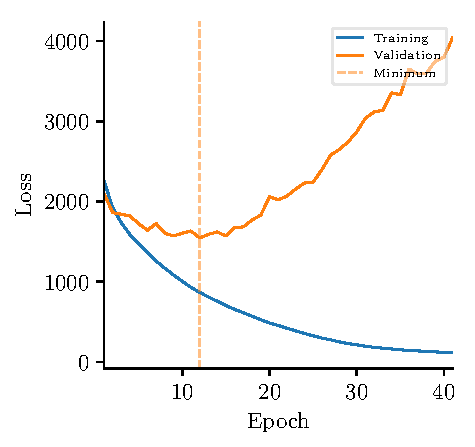
\includegraphics[width=3in]{figures/results/losses/ctc-events}
    \caption{CTC}
  \end{subfigure}
  \caption{}
  \label{fig:loss-events}
\end{figure}

\begin{figure}[h]
  \centering
  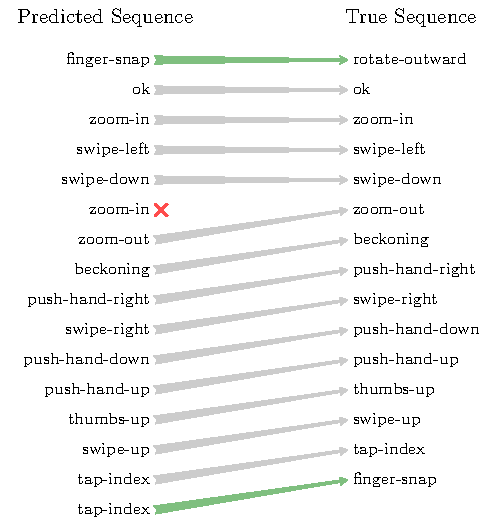
\includegraphics{figures/results/levenshtein}
  \caption{Levenshtein distance of 3}
  \label{fig:levenshtein}
\end{figure}
